\chapter{Results}
\label{cha:results}

%This chapter presents the results. Note that the results are presented
%factually, striving for objectivity as far as possible.  The results
%shall not be analyzed, discussed or evaluated.  This is left for the
%discussion chapter.

%In case the method chapter has been divided into subheadings such as
%pre-study, implementation and evaluation, the result chapter should
%have the same sub-headings. This gives a clear structure and makes the
%chapter easier to write.

%In case results are presented from a process (e.g. an implementation
%process), the main decisions made during the process must be clearly
%presented and justified. Normally, alternative attempts, etc, have
%already been described in the theory chapter, making it possible to
%refer to it as part of the justification.

In this chapter the results are described.
First, the outcome from the exploratory study is presented, followed by the different experiments.
The first experiment, filtering out invalid reports, presents the evaluation of the topic model and k-means model used to filter out the reports, as well as the specific topics and clusters used in the process.
In the second one, the methods considered and the decisions behind which ones that were appropriate are presented.
Finally, the last section goes through the result of evaluating the different active learning techniques.

\section{Exploratory Study}

The goal with the exploratory study was to acquire a better understanding of the data, how it was structured and what kind of information might be extracted from it.
[FIGURE FROM METHOD] displayed popular terms from a subset of the topics obtained from the topic model.
Certain fields such as the cancelled field did not seem to be very reliable. 
Reports that clearly explained a situation where the patient had been transferred to another hospital, or for another reason not having performed an examination, still described a situation where the cancelled field was set to ``false''.
After further manual analysis it was clear that the vast amount of invalid reports were contained within a few topics, something that is used in the first research question.
The evaluation of more concrete relationships were done within the context of that experiment, and is presented in Section~\ref{sec:exp1-result}.

The word2vec model produced results that allowed for synonyms to be detected.
By doing this, 420 pairs were discovered.
The vast majority of these were names, medical terms that (some of which the author was unable to evaluate, and therefore excluded) as well as words that are used in similar contexts, which includes opposites like ``left'' and ``right''.
Disregarding these, the synonyms and misspellings that were decided for use in the final system can be seen in Table~\ref{tab:synonyms}.
The original value was replaced with the new one in the final system.

\begin{table}
    \centering
    \begin{tabular}{|ccc|}
        \hline
        \textbf{Original} & \textbf{Replacement} & \textbf{Type} \\
        \hline
        ordinärt & normalt & synonyms \\
        ej & inte & synonyms \\
        avbeställd & avbokad & synonyms \\
        avebställd & avbokad & misspelling + synonym \\
        belsutat & beslutat & misspelling \\
        måttliga & lätta & synonyms \\
        pat & patient & short \\
        pt & patient & short \\
        pateint & patient & misspelling \\
        akuten & akutmottagningen & misspelling \\
        us & undersökning & short \\
        \hline
    \end{tabular}
    \caption{The synonyms, misspellings and shorts found in the data that the author could with assert with confidence.}
    \label{tab:synonyms}
\end{table}

In order to identify names from this word2vec model, it was plotted using the an interactive plot that allowed for exploring the data.
Since names are commonly used in similar contexts, they would have similar attributes in the word embedding model.
Figure~\ref{fig:word2vec-overview} and Figure~\ref{fig:word2vec-names} show how this was done.
Given that the names got similar coordinates in the plot, identifying the section with names allowed for identification of a lot of the names used in the reports.

\begin{figure}
    \centering
    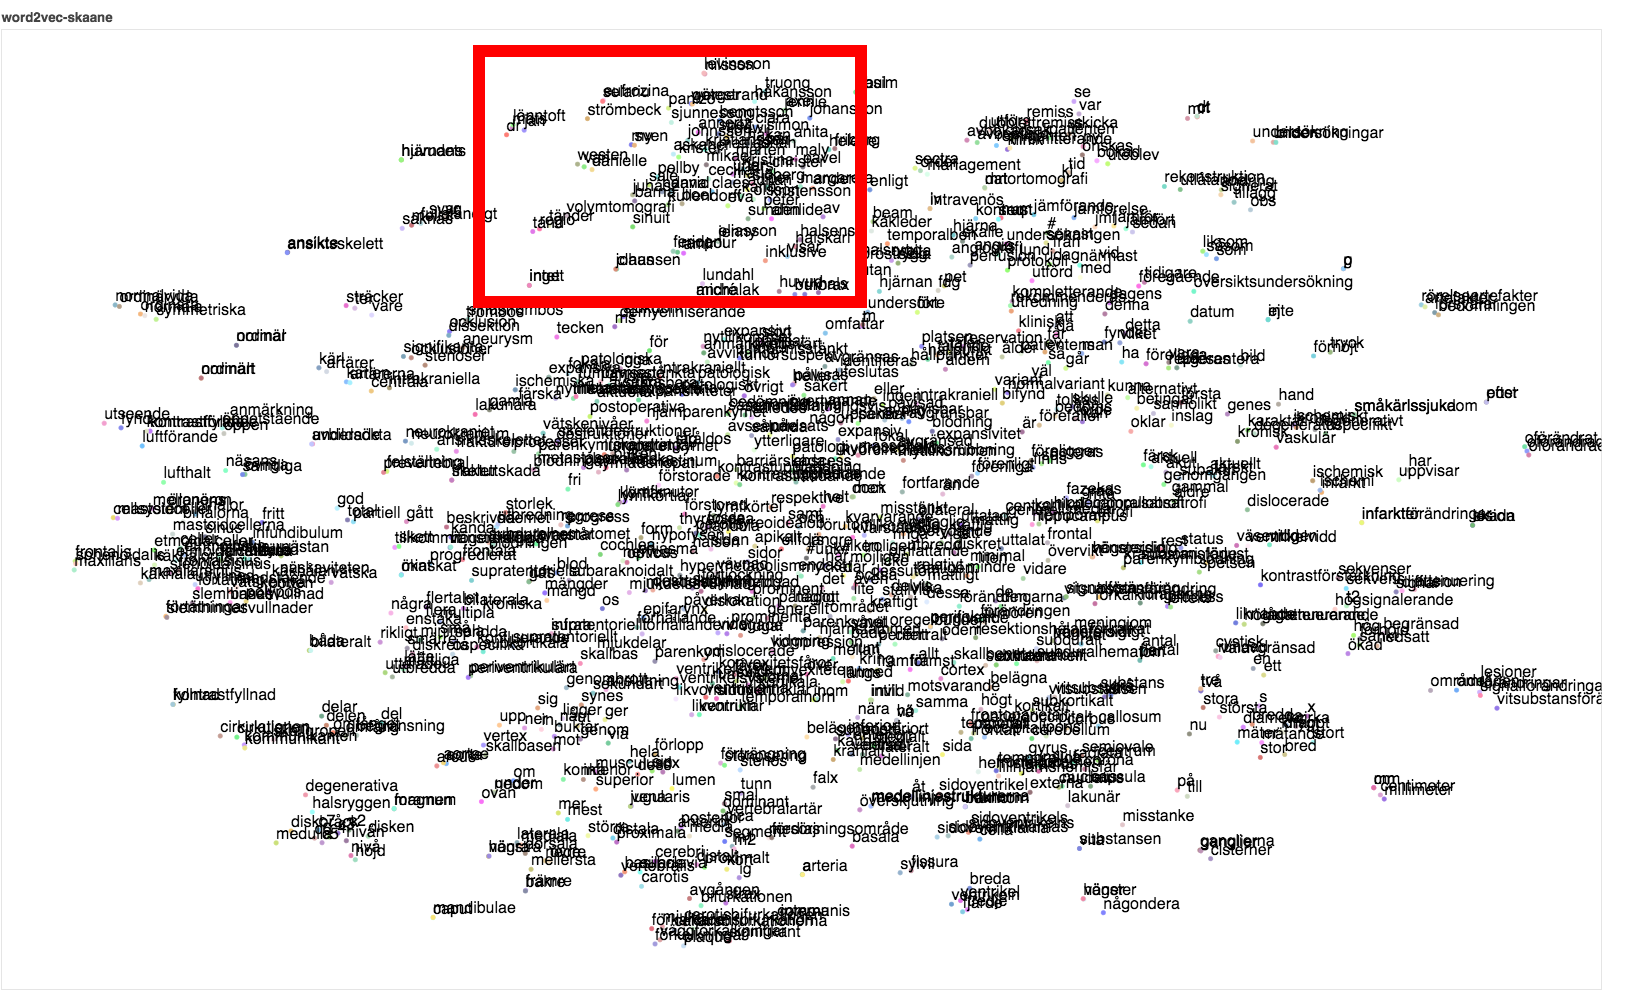
\includegraphics[scale=0.25]{figures/word2vec-overview.png}
    \caption{A 2D plot of the full word2vec plot. Given the amount of terms used there is a lot to analyze.}
    \label{fig:word2vec-overview}
\end{figure}

\begin{figure}
    \centering
    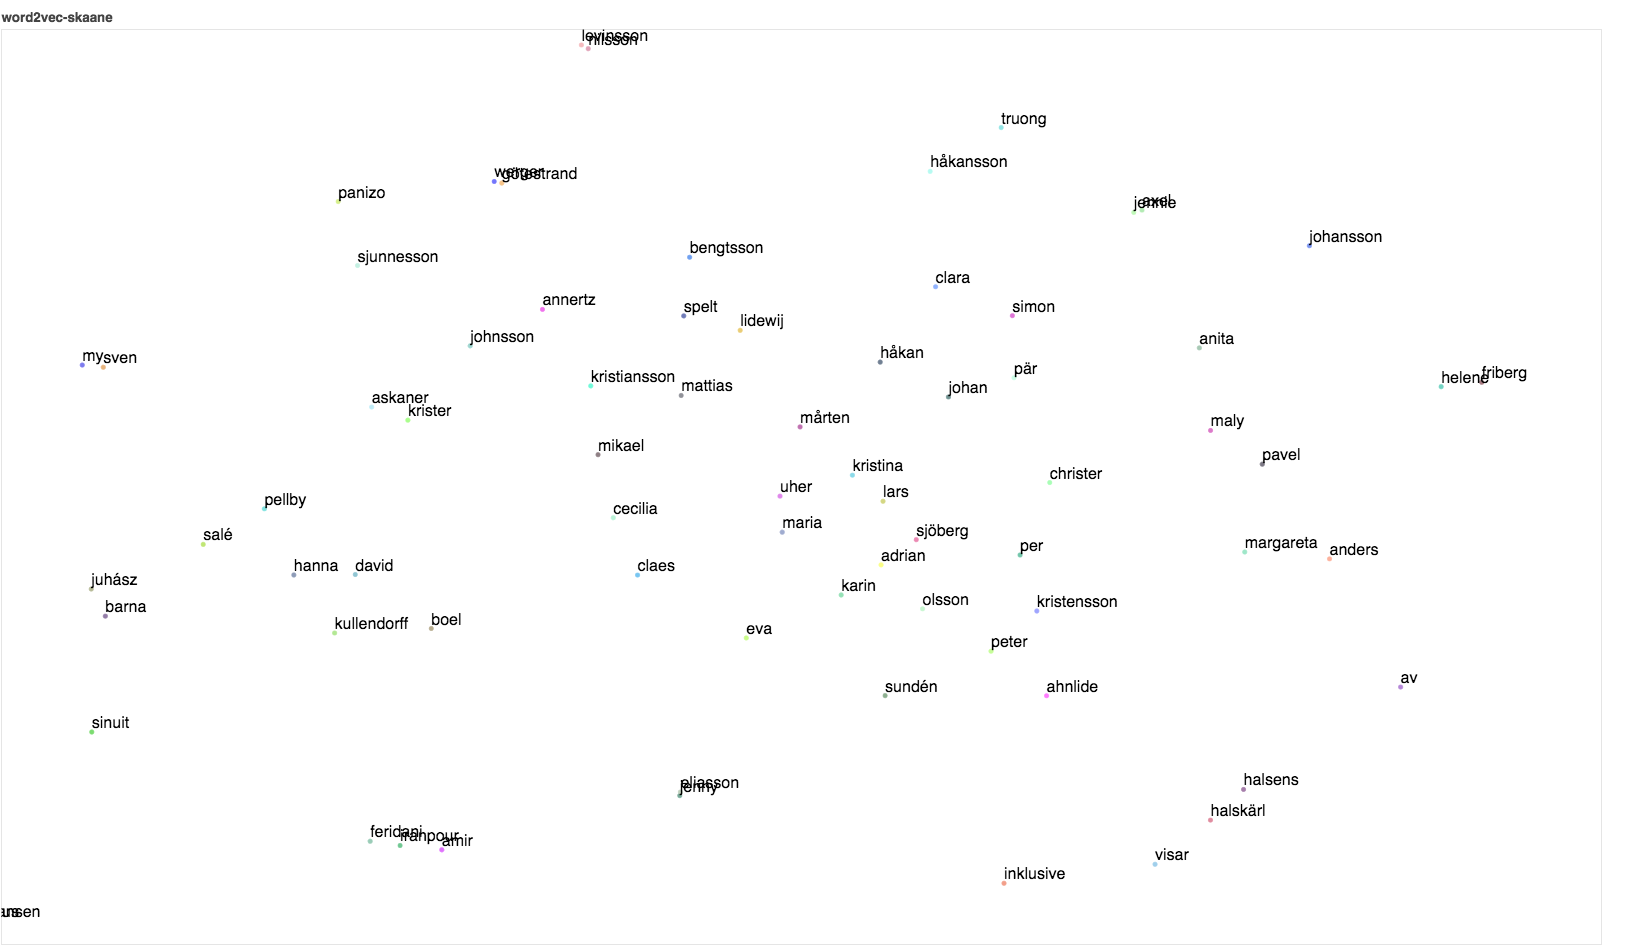
\includegraphics[scale=0.25]{figures/word2vec-names.png}
    \caption{A 2D plot of the zoomed in word2vec plot. Most of the values here are names. This represents the red box zoomed in from Figure~\ref{fig:word2vec-overview}}.
    \label{fig:word2vec-names}
\end{figure}

\section{Filter Out Invalid Clinical Reports Using Topic Models and Clustering}\label{sec:exp1-result}

\textit{Still to be done: Add actual concrete results}

The LDA models were evaluated by calculating the perplexity on the held-out set as described in Section~\ref{sec:exp1-method}.
Perplexity for the evaluated models can be seen in Figure~\ref{fig:lda-perplexity}.
Based on this, the selected model was the LDA model with 75 topics.

\begin{figure}
    \centering
    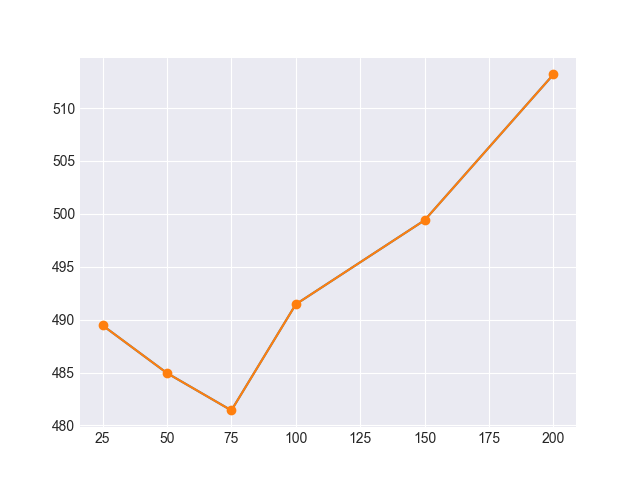
\includegraphics[scale=0.8]{figures/lda-perplexity.png}
    \caption{The perplexity scores for the different LDA models}
    \label{fig:lda-perplexity}
\end{figure}

The next step was identifying the topics that were assigned to the invalid reports.

\begin{figure}
    \centering
    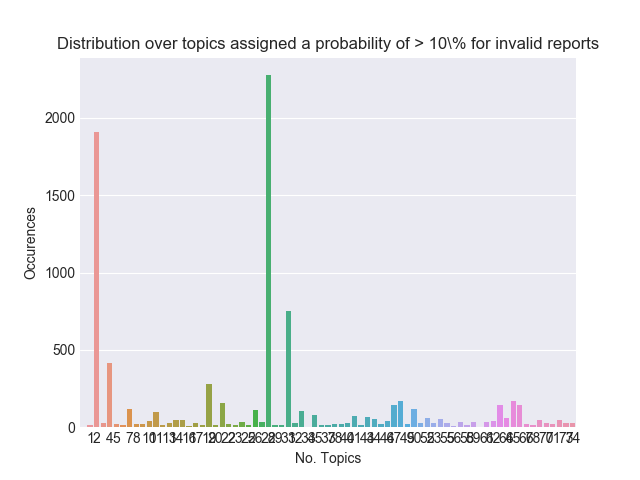
\includegraphics[scale=0.8]{figures/distribution_invalid_reports_likely.png}
    \caption{The distribution of invalid reports that got the topics assigned to them with a probability larger than 10\%}
    \label{fig:invalid-reports-topic-dist-likely}
\end{figure}

\begin{figure}
    \centering
    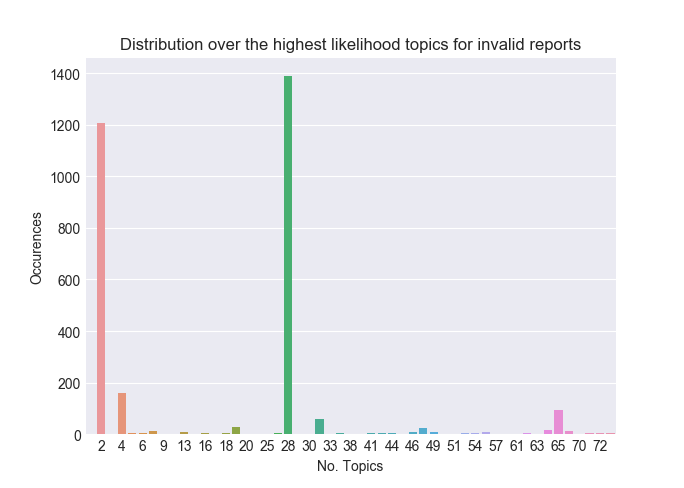
\includegraphics[scale=0.8]{figures/distribution_invalid_reports_highest_likelihood.png}
    \caption{The distribution of invalid reports that got the topics assigned to them with the highest probability}
    \label{fig:invalid-reports-topic-dist-likeliest}
\end{figure}

Each topic that is assigned to a report with a probability above 10\% is considered to be a prominent topic.
The distribution of the most likely topics for the invalid reports can be seen in Figure~\ref{fig:invalid-reports-topic-dist-likely} and Figure~\ref{fig:invalid-reports-topic-dist-likeliest}.
Figure~\ref{fig:invalid-reports-topic-dist-likely} shows the distribution for the different topics where prominent topics for the invalid reports are counted.
Figure~\ref{fig:invalid-reports-topic-dist-likeliest} shows the distribution for the different topics where the topic with the highest probability for each invalid report is counted.
A couple of topics, namely 2 and 28 stands out as the ones with by far the most invalid reports.
But topics 4, 65 and 31 also show significant counts.
In Figure~\ref{fig:invalid-reports-topic-dist-likely} figure a few more topics, such as 19, shows a higher count.

The results of the analysis of the number of prominent topics assigned to each report can be seen in Figure~\ref{fig:no_topics_invalid} and Figure~\ref{fig:no_topics_all}.
Among the invalid reports, the most common number of prominent topic is 2, while it is 6 topics for the entire set of reports.
For the entire set of reports, being assigned 2 topics is the 6th most common number.
This result indicates that there is a relationship between the number of prominent topics assigned to each report, and wether that report is invalid or not.

\begin{figure}
    \centering
    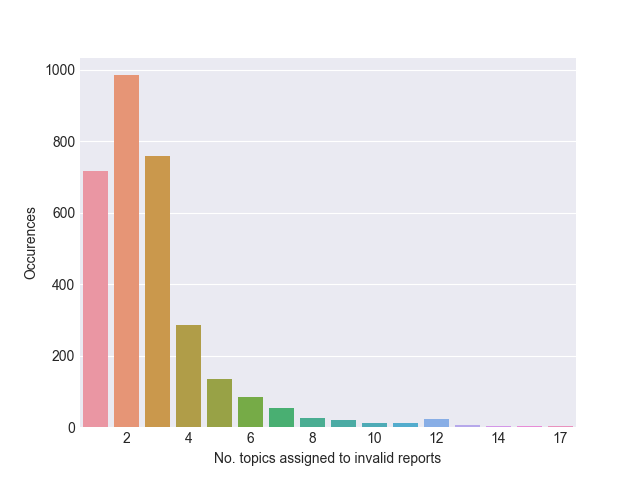
\includegraphics[scale=0.8]{figures/no_topics_per_invalid_report}
    \caption{The distribution of the number of prominent topics assigned to the invalid reports}
    \label{fig:no_topics_invalid}
\end{figure}

\begin{figure}
    \centering
    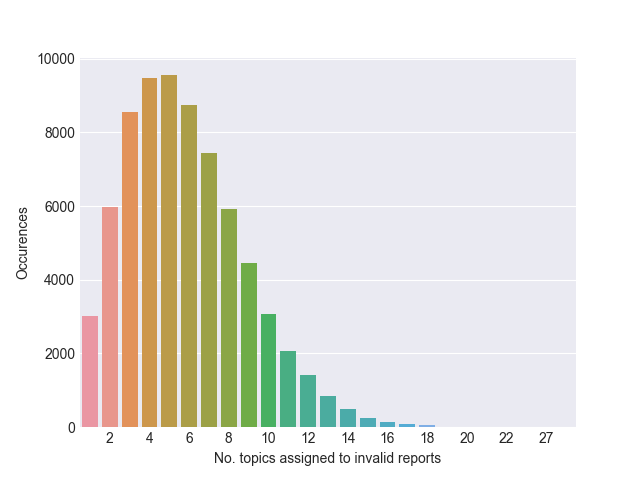
\includegraphics[scale=0.8]{figures/no_topics_per_report}
    \caption{The distribution of the number of prominent topics assigned to the reports}
    \label{fig:no_topics_all}
\end{figure}

Labels were determined to be invalid or not by the following criterion:
\begin{itemize}
    \item Having either topic 2 or 28 among its most probable topic.
    \item Being shorter than 400 characters.
    \item Not having more than 5 prominent topics assigned to it.
\end{itemize}

\textit{The result of this was...}

\section{Alternatives to Labeling at Random}

\textit{Still to be done: Compare the different initial sample sizes (currently same plot)}

The first technique used in this experiment was to explore and try to find a relationship between the initial set of labeled data and the inherit structure of it, obtained and visualized with the use of the LDA model.
However, the relationship is not clear enough so that a cluster or topic could simply be mapped to a certain label.
The resulting plot can be seen in Figure~\ref{fig:categories-lda-50}.
From this plot it is clear that there is a grouping of labels.
However, there exists plenty of overlap between different classes.

\begin{figure}
    \centering
    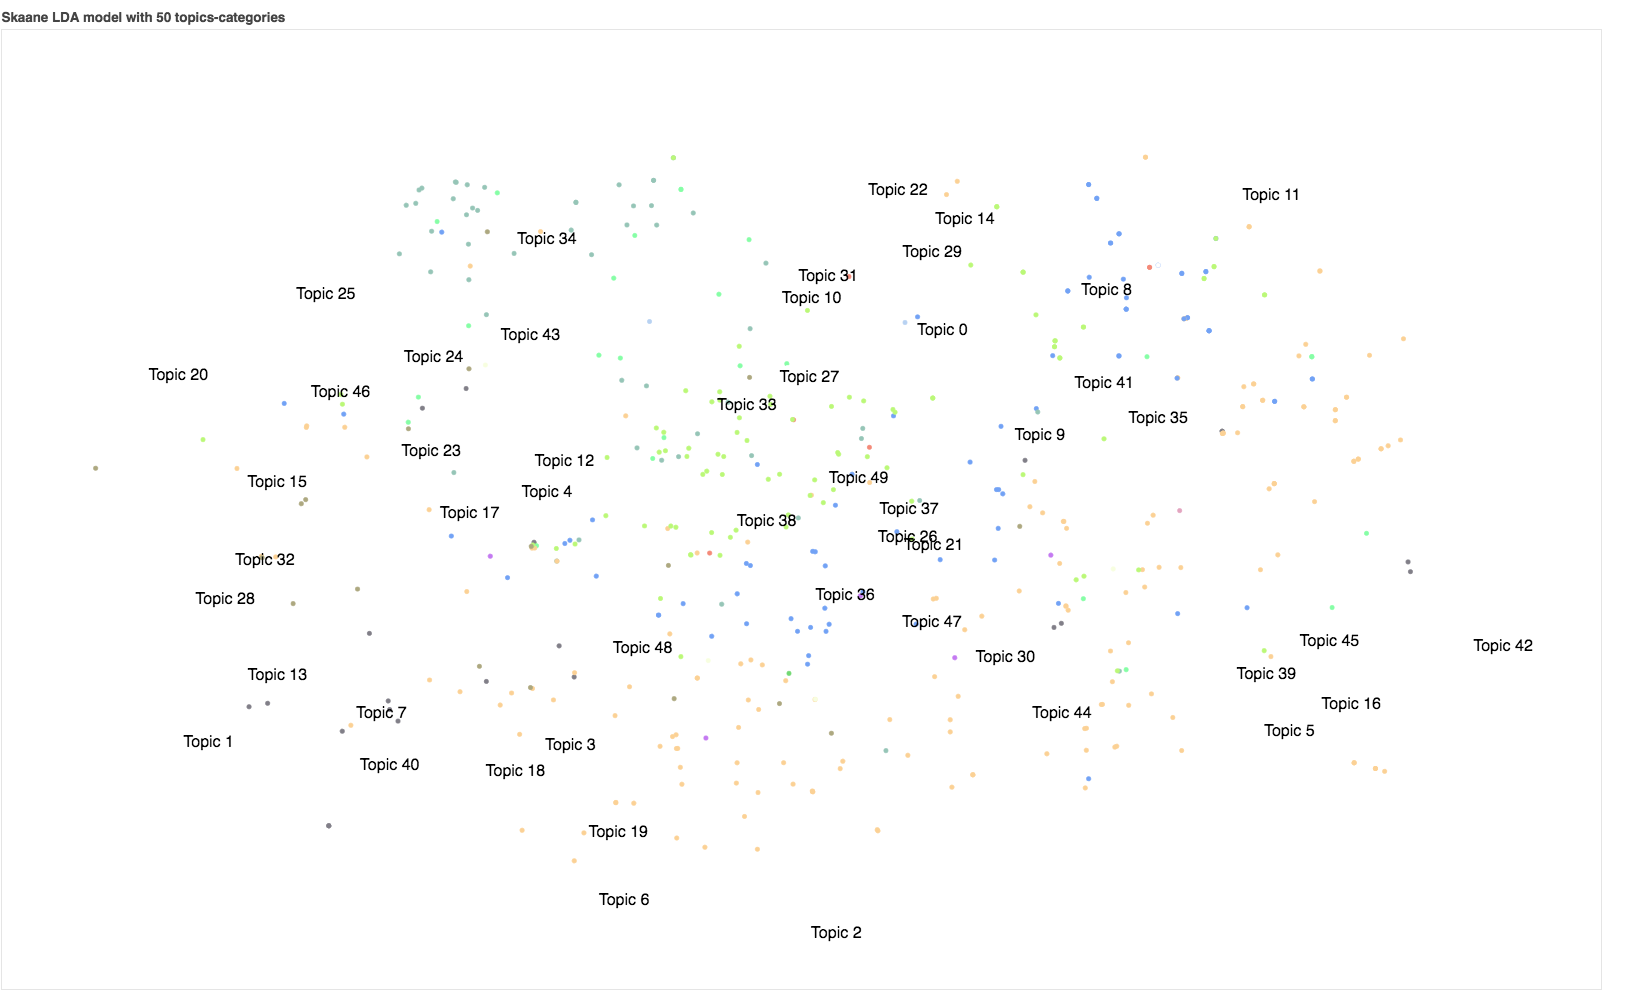
\includegraphics[scale=0.35, angle=270]{figures/categories-lda-50.png}
    \caption{The labeled data points plotted in 2D, and colored based on the first label in alphabetical order.}
    \label{fig:categories-lda-50}
\end{figure}

Based on the knowledge that there exists a pattern, the initial goal was to find some methods that could exploit this.
Some active learning approaches using different forms of clustering, such as Dasgupta et al\@'s approach using hierarchical clustering~\cite{dasgupta2008hierarchical} would be good contenders.
However, the method described by Dasgupta et al\@. is made for the single-label case with no obvious way of extending the technique into multi-label.
The same applies to the density based technique suggested by Attenberg et al\@.~\cite{attenberg2013class}.

Most of the active learning research seems to be focused on binary, or maybe multi-class classification.
Therefor, the methods described in Section~\ref{sec:active-learning} where the ones decided on.
Methods that are fully reliant on a models certainty, such as Binary Version Space Minimization~\cite{brinker2006active} are tested.
In addition to this, methods incorporating some information about the data in the form of label cardinality is included as well.
These techniques are MMC and Adaptive Active Learning~\cite{yang2009effective, li2013active}.
An attempt to take advantage of the structure of the data is done by selecting the initial samples from different clusters, as described in Section~\ref{sec:exp2-method}.

The first metric for evaluation was Accuracy.
A plot of this can be seen in Figure~\ref{fig:al-accuracy-25} to Figure~\ref{fig:al-accuracy-200}.
It contains the accuracy evaluations for the different number of initial sample sizes.
It can easily be seen that the adaptive learner performs significantly better for the first 400 added samples.
However, after that MMC and Binary Version Space Minimization catches up to it, and surpasses it in terms of accuracy after around 800 labels.
Both of them sustaining an significant improvement over labeling at random after round 200 labels.
It takes sampling at random approximately 1600 labels to get to an accuracy of 78\%.
Adaptive Active Learning acquires this accuracy after around 300 labels, and BinaryMinimization and MMC after 450.

\begin{figure}
    \centering
    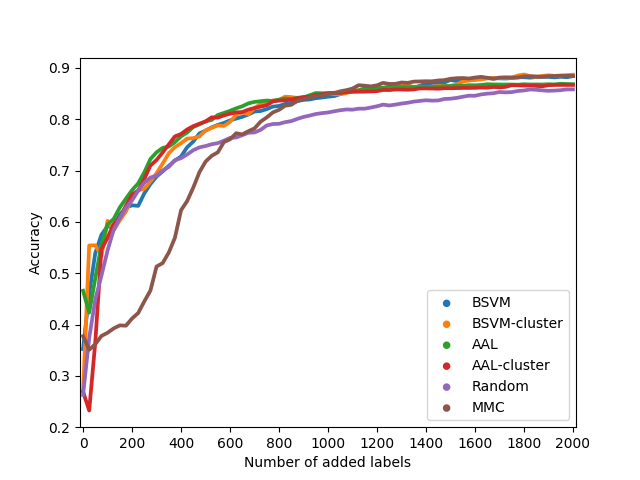
\includegraphics[scale=0.5]{figures/al-25-accuracy.png}
    \caption{Accuracy of the models with initial sample size 25}
    \label{fig:al-accuracy-25}
\end{figure}

When it comes to micro F1-Score, the results between the different methods are similar.
Adaptive Active Learning performs better than the rest in the beginning, but the other active learning strategies obtain similar results after around 500 labels.
One difference from the accuracy evaluation is that Binary Version Space Minimization does not quite surpass the adaptive learner in the same way.
The gap to random sampling is smaller as well.
The results can be seen in Figure~\ref{fig:al-micro-f1-25} to Figure~\ref{fig:al-micro-f1-25}.

\begin{figure}
    \centering
    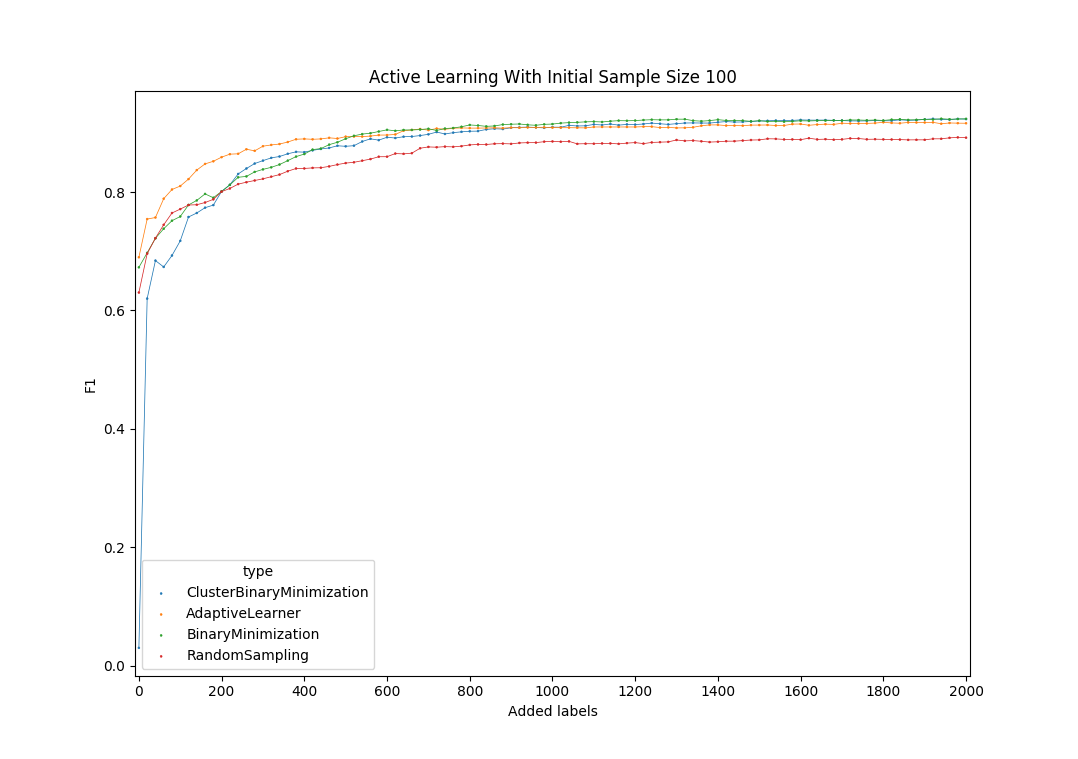
\includegraphics[scale=0.5]{figures/al-25-micro-f1.png}
    \caption{Accuracy of the models with initial sample size 25}
    \label{fig:al-micro-f1-25}
\end{figure}

The same applies to micro recall.
The one difference is that the Adaptive Active Learner strategy is performing better than the rest for more iterations.
It takes approximately 1000 added labels for the BinaryMinimization to obtain similar micro recall.
This can be seen in Figure~\ref{fig:al-micro-fig:al-micro-recall-25}.
The random sampling performs considerably worse than the rest.

\begin{figure}
    \centering
    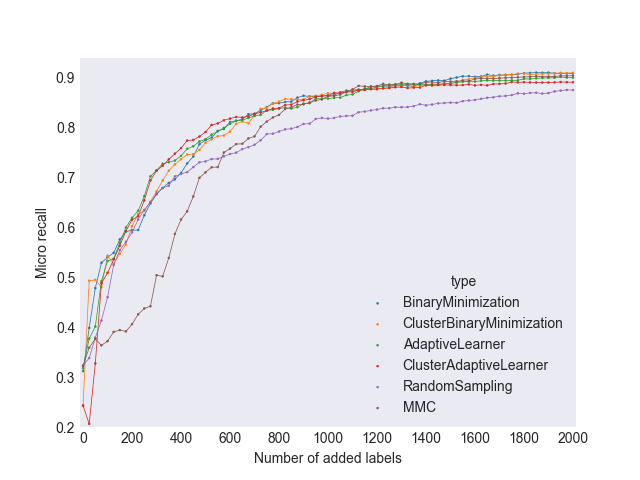
\includegraphics[scale=0.5]{figures/al-25-micro-recall.png}
    \caption{Micro recall of the models with initial sample size 25}
    \label{fig:al-micro-recall-25}
\end{figure}

The micro precision of the models are very similar between all strategies.
Algorithms using clustering obtains a higher precision between 200-400 added labels, but not by that much.
From 200 added labels and onwards, Adaptive Active Learner is worse than Binary Version Space Minimization.

\begin{figure}
    \centering
    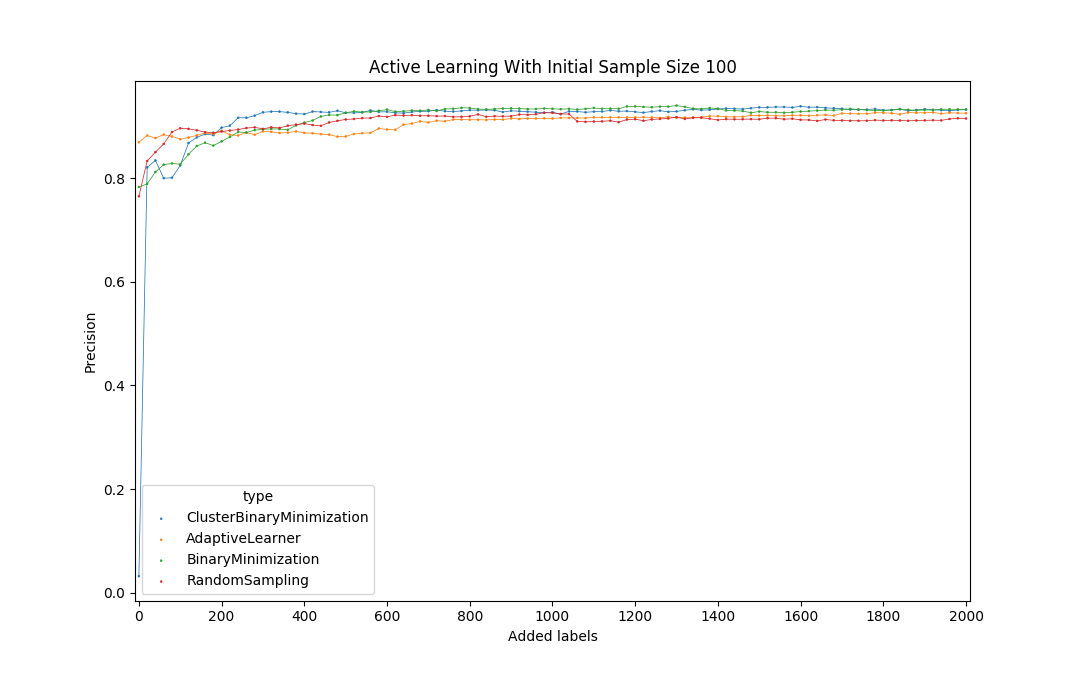
\includegraphics[scale=0.5]{figures/al-100-micro-precision.png}
    \caption{Micro precision of the models with initial sample size 25}
    \label{fig:al-micro-precision-25}
\end{figure}

Another important aspect of the evaluation is the time it takes.
This can be seen in Figure~\ref{fig:al-time}.
Time is constant for the random sampling, very close to 0.
For the Binary Minimization, the time increases a bit every iteration, but stays under 200 seconds for the first samples.
MMC gets similar results, but takes a bit longer.
The Adaptive Active Learner takes far longer time than the other methods.

\begin{figure}
    \centering
    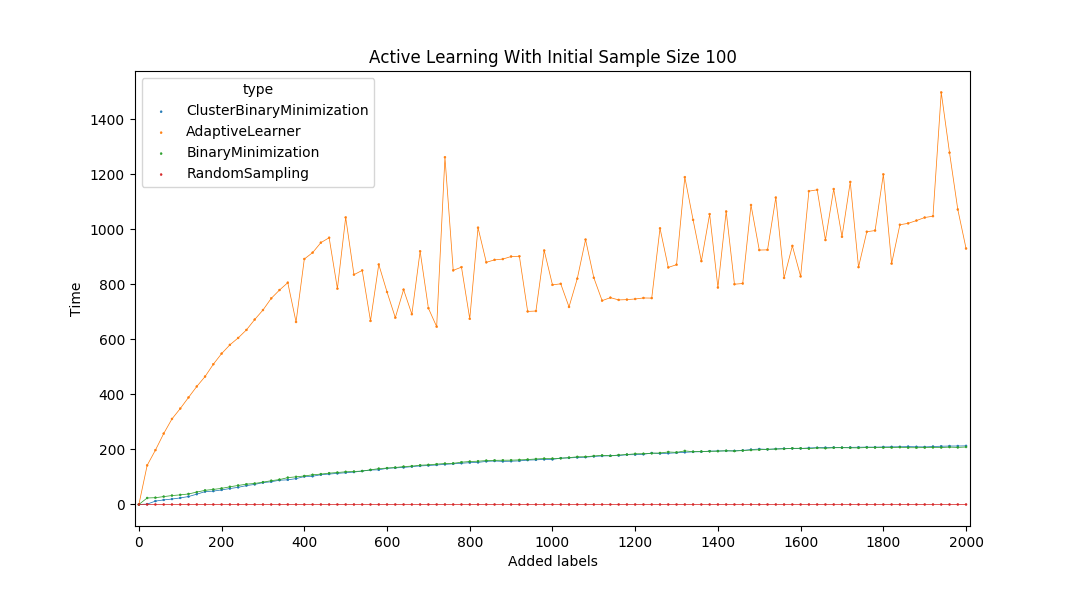
\includegraphics[scale=0.5]{figures/al-time.png}
    \caption{Time to query a new set of samples by the different strategies}
    \label{fig:al-micro-precision-25}
\end{figure}


\section{Evaluating the Label Balance}

The last part to evaluate is how the different Active Learning techniques effected the balance of the labels.
For the Reuters dataset, how the overall distribution of the labels is can be seen in Figure~\ref{fig:class-distribution-reuters}.
After random sampling, the distribution can be seen in Figure~\ref{fig:class-distribution-reuters-random}.
The distribution after sampling with the original Binary Version Space Minimization can be seen in Figure~\ref{fig:class-distribution-reuters-binmin}, and with the initial samples taken from clusters in Figure~\ref{fig:class-distribution-reuters-binmin-clusters}.
The ratio between the biggest and smallest class is here $X_1$ compared to $X_2$ for the random sampling.
When the initial labeled set was selected from the clusters, the ratio was $X$.
For MMC the distribution can be seen in Figure~\ref:fig:class-distribution-reuters-mmc}, and for Adaptive Active Learning in Figure~\ref{fig:calss-distribution-reuters-adaptive}.
The imbalance ratio between the biggest and the smallest class here is $X_1$ and $X_2$, respectively.
Figure~\ref:fig:class-distribution-reuters-mmc-clusters} and Figure~\ref:fig:class-distribution-reuters-adaptive-clusters} shows the distribution for the same methods, but with the initial samples taken from the clusters.

\begin{figure}
    \centering
    \thirdsubfigimg{reuters-random-distribution-20}{The class distribution from random sampling after 200 labels}
    \thirdsubfigimg{reuters-random-distribution}{The class distribution from random sampling after 2000 labels}
    \caption{The distribution of labels after random sampling}
    \label{fig:class-distribution-reuters-random}
\end{figure}

\begin{figure}
    \centering
    \thirdsubfigimg{reuters-binmin-distribution-20}{The class distribution from Binary Version Space Minimization after 200 labels}
    \thirdsubfigimg{reuters-binmin-distribution}{The class distribution from Binary Version Space Minimization after 2000 labels}
    \caption{The distribution of labels after Binary Version Space Minimization}
    \label{fig:class-distribution-reuters-binmin}
\end{figure}


\begin{figure}
    \centering
    \thirdsubfigimg{reuters-clusterbinmin-distribution-20}{The class distribution from Binary Version Space Minimization with clustering after 200 labels}
    \thirdsubfigimg{reuters-clusterbinmin-distribution}{The class distribution from Binary Version Space Minimization with clusterinp after 2000 labels}
    \caption{The distribution of labels after Binary Version Space Minimization with clustering}
    \label{fig:class-distribution-reuters-binmin-clusters}
\end{figure}

\begin{figure}
    \centering
    \thirdsubfigimg{reuters-adaptive-distribution-20}{The class distribution from Adaptive Active Learning after 200 labels}
    \thirdsubfigimg{reuters-adaptive-distribution}{The class distribution from Adaptive Active Learning after 2000 labels}
    \caption{The distribution of labels after Adaptive Active Learning}
    \label{fig:class-distribution-reuters-binmin-clusters}
\end{figure}